\section{Proposed Solution}

The proposed solution is a modular, AI-based platform in which each module analyses one kind of security evidence and returns a structured finding. The platform is designed around two complementary ideas. \textit{Supervised} models give precise labels for threats they have learned, while an \textit{unsupervised} anomaly detector covers behaviour that no model has seen before. Their outputs are then meant to be combined, correlated and explained to the analyst. This section describes the overall architecture, the three implemented modules with their current results, the remaining planned components, and the main design considerations.

\subsection{System Architecture and Workflow}

Figure~\ref{fig:architecture} shows the intended architecture. Solid boxes are components that have been implemented and evaluated, the dashed orange box is the log analysis module now in development, and dashed grey boxes are planned components. The intended workflow is as follows:
\begin{enumerate}[itemsep=1pt, topsep=2pt]
  \item Security evidence enters the platform: network flow records, PE malware feature vectors and logs.
  \item Each analysis module processes the evidence it is responsible for and produces a structured result, such as a class label with confidence, or an alert with a severity level and explanation.
  \item The planned backend stores these results and passes them to the correlation, risk and investigation components.
  \item The dashboard presents incidents, risk levels and explanations to the analyst, whose feedback is recorded to evaluate and improve the system.
\end{enumerate}
At the mid-term stage, steps 1 and 2 are implemented for the three completed modules, which run as standalone prototypes on benchmark data. Steps 3 and 4 are planned.

\begin{figure}[htbp]
\centering
\resizebox{\textwidth}{!}{%
\begin{tikzpicture}[node distance=6mm and 8mm]
  % inputs
  \node[data] (flows) {Network flow\\records (CSV)};
  \node[data, below=10mm of flows] (pe) {PE malware\\feature vectors};
  \node[data, below=10mm of pe] (logs) {System and\\application logs};
  % modules
  \node[done, right=14mm of flows, yshift=8mm, text width=36mm] (ntc) {\textbf{Network Threat}\\\textbf{Classification}\\two-stage LightGBM};
  \node[done, below=4mm of ntc, text width=36mm] (ad) {\textbf{Anomaly Detection}\\unsupervised ensemble};
  \node[done, right=14mm of pe, yshift=-6mm, text width=36mm] (mw) {\textbf{Malware}\\\textbf{Classification}\\CatBoost + Random Forest};
  \node[wip, right=14mm of logs, text width=36mm] (log) {\textbf{Log Analysis}\\(in progress)};
  \draw[arr] (flows.east) -- (ntc.west);
  \draw[arr] (flows.east) -- (ad.west);
  \draw[arr] (pe.east) -- (mw.west);
  \draw[darr] (logs.east) -- (log.west);
  % outputs
  \node[box, right=12mm of ad, yshift=-10mm, text width=34mm] (out) {Structured findings:\\labels, confidence,\\severity, top features};
  \draw[arr] (ntc.east) -- (out);
  \draw[arr] (ad.east) -- (out);
  \draw[arr] (mw.east) -- (out);
  \draw[darr] (log.east) -- (out);
  % planned layer
  \node[plan, right=12mm of out, text width=34mm] (api) {Backend API\\and database};
  \node[plan, above=6mm of api, text width=34mm] (corr) {Incident correlation\\and risk analysis};
  \node[plan, below=6mm of api, text width=34mm] (agent) {Investigation\\agent};
  \node[plan, right=10mm of api, text width=26mm] (dash) {Dashboard\\and feedback};
  \node[box, right=8mm of dash, text width=14mm] (user) {Analyst};
  \draw[darr] (out) -- (api);
  \draw[darr] (api) -- (corr);
  \draw[darr] (api) -- (agent);
  \draw[darr] (corr.east) -| (dash.north);
  \draw[darr] (agent.east) -| (dash.south);
  \draw[darr] (api) -- (dash);
  \draw[darr] (dash) -- (user);
  % legend
  \node[done, below=14mm of agent, xshift=-22mm, minimum height=5mm, font=\scriptsize] (l1) {Completed};
  \node[wip, right=3mm of l1, minimum height=5mm, font=\scriptsize] (l2) {In progress};
  \node[plan, right=3mm of l2, minimum height=5mm, font=\scriptsize] (l3) {Planned};
\end{tikzpicture}}
\caption{Overall architecture of the AI-Based Autonomous Cyber Defense System and implementation status at mid-term}
\label{fig:architecture}
\end{figure}

The three completed modules do not yet exchange data with each other. They were developed independently, each by one team member, and they share a design principle: every module produces machine-readable output that the planned backend can consume. The network and anomaly modules both analyse flow records but answer different questions. The network module asks \textit{which known attack does this flow resemble?}, while the anomaly module asks \textit{how unusual is this flow compared with normal traffic?} Section~\ref{sec:module-relationship} discusses how the two are expected to complement each other.

\subsection{Module 1: Network Threat Classification}

\textbf{Role.} This module labels network flows as benign or as one of six attack families, so that the analyst sees what kind of activity is taking place, not just that something is wrong.

\textbf{Dataset.} The module uses the CIC-IDS2017 dataset published by the Canadian Institute for Cybersecurity \cite{sharafaldin2018cicids,cicids2017web}. It contains five days of benign and attack traffic, recorded as flows by the CICFlowMeter tool. All eight flow files were used, giving 2,830,743 usable flows described by 77 numeric features. Source and destination addresses, ports and timestamps were excluded so that the model cannot rely on identifiers. The original labels were grouped into seven classes (Table~\ref{tab:ntc-data}). In the module's taxonomy, the \textit{WebAttack} group also contains the FTP-Patator and SSH-Patator brute-force attacks and the Heartbleed exploit. The data is highly imbalanced: about 80.3\% of flows are benign, and only 36 Infiltration flows exist in the entire dataset.

\begin{table}[H]
\centering
\caption{Class distribution of the prepared CIC-IDS2017 data used by the Network Threat Classification module}
\label{tab:ntc-data}
\small
\begin{tabular}{lrrr}
\toprule
\textbf{Class} & \textbf{All rows} & \textbf{Train rows} & \textbf{Test rows} \\
\midrule
BENIGN       & 2,273,097 & 1,826,507 & 446,590 \\
DoS          &   252,661 &   206,951 &  45,710 \\
PortScan     &   158,930 &   129,834 &  29,096 \\
DDoS         &   128,027 &   102,360 &  25,667 \\
WebAttack    &    16,026 &    13,048 &   2,978 \\
Botnet       &     1,966 &     1,582 &     384 \\
Infiltration &        36 &        29 &       7 \\
\midrule
Total        & 2,830,743 & 2,280,311 & 550,432 \\
\bottomrule
\end{tabular}
\end{table}

\textbf{Method.} Preprocessing converts all features to numbers, replaces infinite values, imputes missing values with the training median, removes low-variance features and applies robust scaling. Each step is fitted on training data only, to avoid information leakage. The split keeps identical feature vectors in the same partition, using a fingerprint of selected flow fields. The classifier is a two-stage cascade of LightGBM gradient-boosted tree models \cite{ke2017lightgbm} (Figure~\ref{fig:ntc-flow}). Stage~1 decides between benign and attack, using a decision threshold of 0.7723 chosen on a validation subset. Flows predicted as attacks pass to Stage~2, which assigns one of the six families. Both models use balanced class weights instead of oversampling. Their settings are a learning rate of 0.05, 31 leaves, a minimum of 30 samples per leaf, 85\% feature and row sampling, and L1 and L2 regularisation of 0.1 and 2.0. Early stopping on a validation subset selected 600 trees for Stage~1, which is the configured maximum, and 256 trees for Stage~2. The module also attaches an Isolation Forest anomaly score, a feature-importance explanation, MITRE ATT\&CK context \cite{strom2018attack} and a recommended response plan to each decision. The response plan is produced as text only and is never executed.

\begin{figure}[H]
\centering
\begin{tikzpicture}[node distance=5mm and 7mm, every node/.style={font=\small}]
  \node[data] (in) {Flow record\\(77 features)};
  \node[done, right=of in, text width=24mm] (pre) {Preprocessing\\impute, filter, scale};
  \node[done, right=of pre, text width=22mm] (s1) {Stage 1\\LightGBM\\benign / attack};
  \node[box, above right=2mm and 8mm of s1, text width=18mm] (ben) {BENIGN};
  \node[done, below right=2mm and 8mm of s1, text width=24mm] (s2) {Stage 2\\LightGBM\\6 attack families};
  \node[box, right=6mm of s2, text width=26mm] (out) {Decision with\\confidence, MITRE\\context, response plan};
  \draw[arr] (in) -- (pre);
  \draw[arr] (pre) -- (s1);
  \draw[arr] (s1.east) -- node[above, font=\scriptsize, sloped] {$p<0.7723$} (ben.west);
  \draw[arr] (s1.east) -- node[below, font=\scriptsize, sloped] {$p\geq0.7723$} (s2.west);
  \draw[arr] (s2) -- (out);
\end{tikzpicture}
\caption{Two-stage workflow of the Network Threat Classification module}
\label{fig:ntc-flow}
\end{figure}

\textbf{Results.} The cascade was evaluated once on the 550,432-flow holdout set (Table~\ref{tab:ntc-results}). The binary gate reached 99.70\% attack precision and 99.84\% attack recall. Of the 446,590 benign test flows, 313 were wrongly flagged, and of the 103,842 attack flows, 164 were missed. The end-to-end cascade achieved 99.91\% accuracy with a macro F1-score of 0.9578. The gap between this value and the weighted F1-score of 0.9991 reflects weaker results on rare classes. Botnet recall is 71.35\% (274 of 384 test flows), and the Infiltration result of six correct out of seven is too small to be statistically reliable. Figure~\ref{fig:ntc-cm} shows the confusion matrices.

\begin{table}[H]
\centering
\caption{Holdout performance of the Network Threat Classification module (CIC-IDS2017)}
\label{tab:ntc-results}
\small
\begin{tabular}{lrrrr}
\toprule
\textbf{Evaluation} & \textbf{Rows} & \textbf{Accuracy} & \textbf{Macro F1} & \textbf{Weighted F1} \\
\midrule
Stage 1 (benign vs.\ attack) & 550,432 & 99.91\% & 0.9986 & 0.9991 \\
Stage 2 on true attacks only & 103,842 & 99.98\% & 0.9997 & 0.9998 \\
End-to-end cascade & 550,432 & 99.91\% & 0.9578 & 0.9991 \\
\bottomrule
\end{tabular}
\end{table}

\begin{figure}[htbp]
\centering
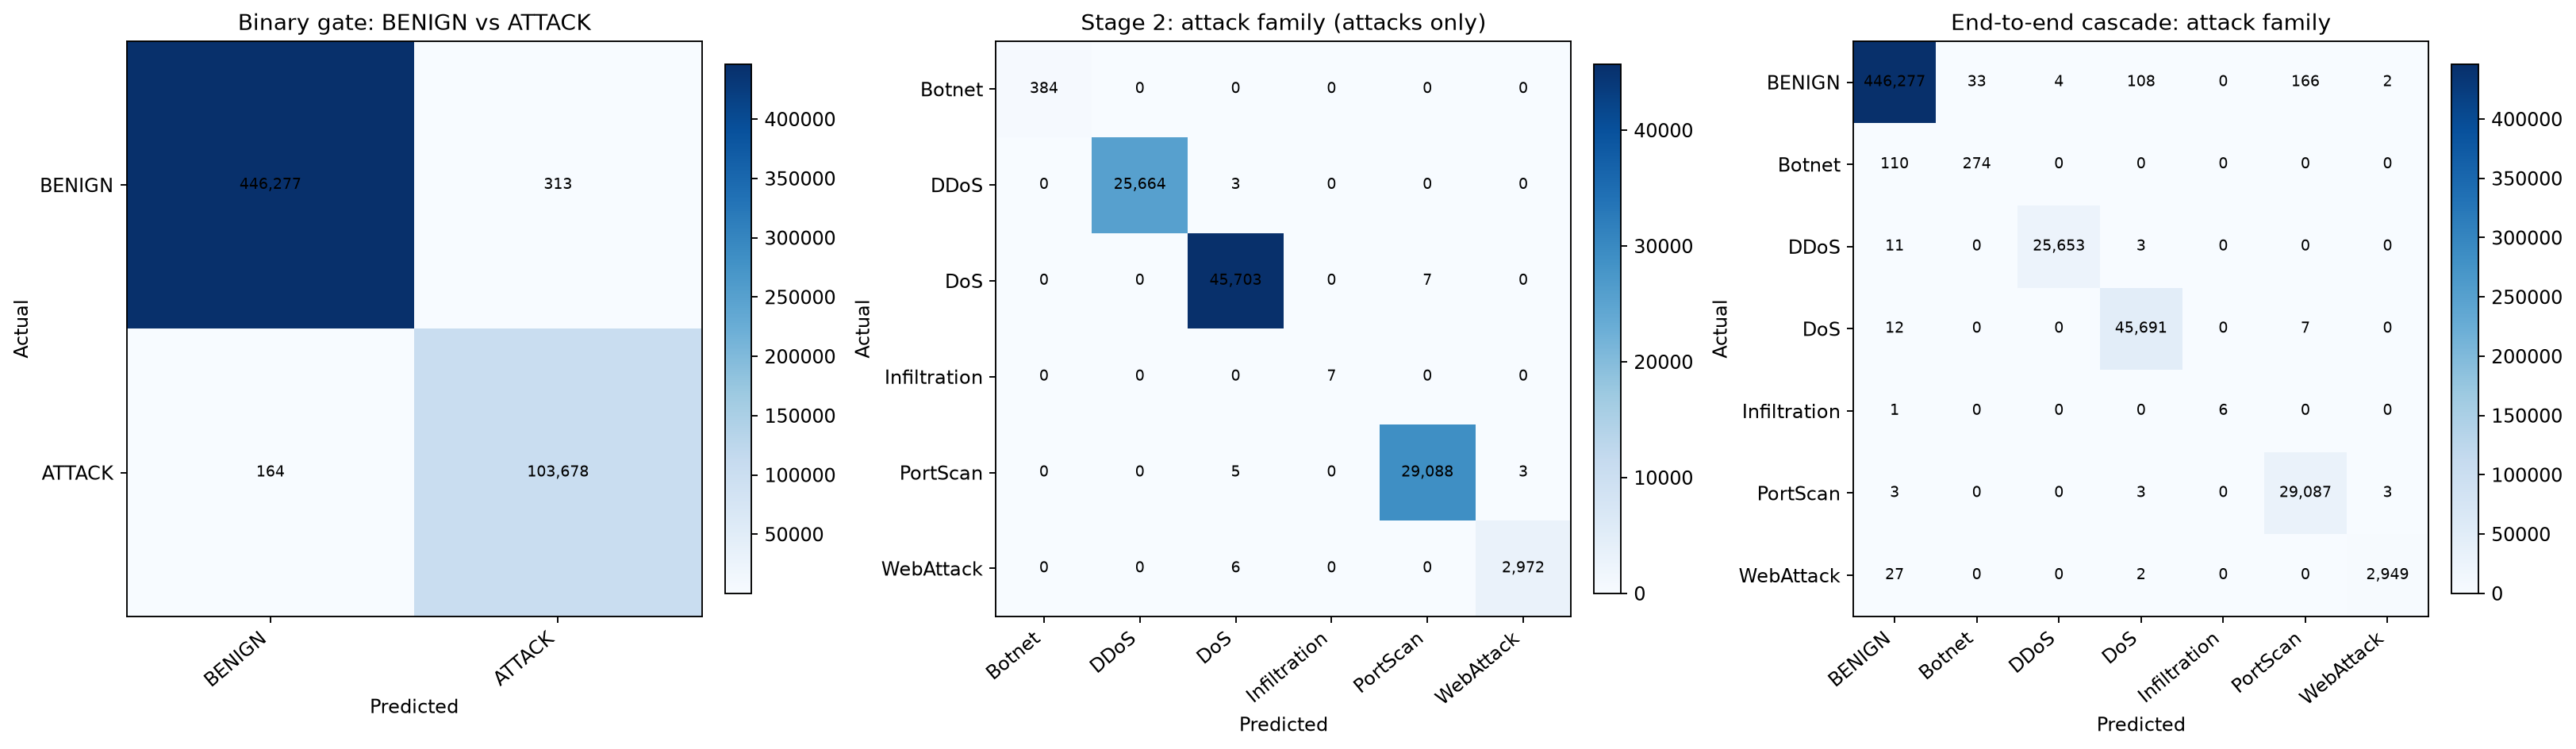
\includegraphics[width=\textwidth]{ntc_eda_4.png}
\caption{Confusion matrices of the Network Threat Classification module on the holdout set: binary gate (left), Stage~2 on true attacks (centre) and end-to-end cascade (right)}
\label{fig:ntc-cm}
\end{figure}

\textbf{Limitations.} CIC-IDS2017 was recorded in a single laboratory network over five days, so these results do not show how the model would perform on a different network or on future traffic. Previous work has also reported labelling and flow-construction problems in this dataset \cite{engelen2021troubleshooting}. The rare classes (Botnet and Infiltration) have too few examples for reliable estimates. Stage~1 used the maximum number of trees allowed, so a wider search might improve it. The attached Isolation Forest score has not been validated against labelled data and is not presented as a detector of new attacks. The current interface is a command-line tool and Python API; live packet capture and response execution are outside the verified scope.

\subsection{Module 2: Malware Classification}

\textbf{Role.} This module decides whether a Windows executable is benign or malicious and, if it is malicious, which category of malware it belongs to. This tells the analyst both whether a file is dangerous and what kind of behaviour to expect from it.

\textbf{Dataset.} The module uses BODMAS, a dataset of Windows PE samples released for research on learning-based malware analysis \cite{yang2021bodmas}. The cleaned version used contains 134,428 samples (77,138 benign and 57,290 malicious), each described by 2,326 numerical static features. The feature format follows the EMBER feature set \cite{anderson2018ember}. Category labels were joined to the malicious samples, and eight categories were selected for the second stage (Table~\ref{tab:mw-data}). Very small categories were left out.

\begin{table}[H]
\centering
\caption{Malware categories used by the second stage of the Malware Classification module (BODMAS)}
\label{tab:mw-data}
\small
\begin{tabular}{lr@{\hspace{3em}}lr}
\toprule
\textbf{Category} & \textbf{Samples} & \textbf{Category} & \textbf{Samples} \\
\midrule
Trojan     & 29,972 & Ransomware          & 821 \\
Worm       & 16,695 & Dropper             & 715 \\
Backdoor   &  7,331 & Information stealer & 447 \\
Downloader &  1,031 & Virus               & 192 \\
\bottomrule
\end{tabular}
\end{table}

\textbf{Method.} Both stages use a stratified 80/20 train--test split with a fixed random seed of 42 (Figure~\ref{fig:mw-flow}). No feature scaling is applied, which suits tree-based models, and no synthetic oversampling such as SMOTE was used. Stage~1 is a CatBoost gradient-boosting classifier \cite{prokhorenkova2018catboost} with 300 iterations, depth 6 and a learning rate of 0.1. Stage~2 is a Random Forest \cite{breiman2001rf} with 100 trees, square-root feature sampling, at least two samples per leaf, and \texttt{balanced\_subsample} class weighting to reduce the effect of category imbalance. A Gradio interface \cite{abid2019gradio} loads the saved models, accepts a CSV file containing the 2,326 features, and displays predictions, confusion matrices and summary charts.

\begin{figure}[H]
\centering
\begin{tikzpicture}[node distance=5mm and 7mm, every node/.style={font=\small}]
  \node[data] (in) {CSV with 2,326\\PE features};
  \node[done, right=of in, text width=24mm] (s1) {Stage 1\\CatBoost\\benign / malware};
  \node[box, above right=2mm and 8mm of s1, text width=18mm] (ben) {Benign};
  \node[done, below right=2mm and 8mm of s1, text width=24mm] (s2) {Stage 2\\Random Forest\\8 categories};
  \node[box, right=6mm of s2, text width=24mm] (out) {Malware category\\shown in Gradio\\interface};
  \draw[arr] (in) -- (s1);
  \draw[arr] (s1.east) -- (ben.west);
  \draw[arr] (s1.east) -- node[below, font=\scriptsize, sloped] {malware} (s2.west);
  \draw[arr] (s2) -- (out);
\end{tikzpicture}
\caption{Two-stage workflow of the Malware Classification module}
\label{fig:mw-flow}
\end{figure}

\textbf{Results.} Table~\ref{tab:mw-results} lists the results reported in the module's documentation. On the 26,886-sample test set, the CatBoost detector misclassified 62 benign samples as malware and missed 71 malicious samples. The Random Forest category classifier reached 94.34\% accuracy and a macro F1-score of 0.8766. The lower macro value reflects weaker results on small categories, especially Virus, which has only 192 samples in the whole dataset.

\begin{table}[H]
\centering
\caption{Test results of the Malware Classification module (as reported in the module documentation)}
\label{tab:mw-results}
\small
\begin{tabular}{llr}
\toprule
\textbf{Stage} & \textbf{Metric} & \textbf{Value} \\
\midrule
\multirow{5}{*}{Stage 1: CatBoost (benign vs.\ malware)}
 & Accuracy              & 99.51\% \\
 & Precision (malware)   & 99.46\% \\
 & Recall (malware)      & 99.38\% \\
 & F1-score (malware)    & 99.42\% \\
 & ROC-AUC               & 99.97\% \\
\midrule
\multirow{3}{*}{Stage 2: Random Forest (8 categories)}
 & Accuracy              & 94.34\% \\
 & Macro F1-score        & 87.66\% \\
 & Weighted F1-score     & 94.32\% \\
\bottomrule
\end{tabular}
\end{table}

\textbf{Limitations.} The module classifies pre-extracted feature vectors. It does not yet extract features from raw executable files, scan endpoints in real time, or quarantine files. The Stage~2 result was measured on samples already known to be malicious, so it shows how well categories are separated, not the error of the full two-stage pipeline. The two stages were also evaluated on separate splits. Metrics from earlier experiments, such as a CatBoost run with 99.00\% accuracy, are not part of the final pipeline. The values in Table~\ref{tab:mw-results} must be re-confirmed against the saved metrics file before the final report. Finally, malware evolves over time, and a random split may overestimate performance on future samples. Temporal evaluation, which BODMAS was designed to support \cite{yang2021bodmas}, is left for future work.

\subsection{Module 3: Anomaly Detection}

\textbf{Role.} This module detects network activity that deviates from normal behaviour, whether or not it matches a known attack. It is trained only on benign traffic, so it needs no attack labels to learn and can flag attack types that the supervised classifiers have never seen \cite{chandola2009anomaly,ahmed2016anomaly}. Each alert includes a severity level and the features that were most abnormal, so that the analyst can see why it was raised.

\textbf{Datasets and protocol.} The module was evaluated on NSL-KDD \cite{tavallaee2009nslkdd} and CIC-IDS2017 \cite{sharafaldin2018cicids}. NSL-KDD uses its official training and test files. Its test file contains 17 attack types (3,750 of 12,833 attack records) that never appear in training, which makes it a direct test of detecting unseen attacks. For CIC-IDS2017, an analysis found that 10.9\% of all rows (23.6\% of attack rows) are exact duplicates, and 1,396 rows have identical features but conflicting labels. Duplicate flows split across training and test sets would inflate results. The module therefore removes duplicates and conflicting rows before splitting, then draws a fixed 10\% sample and splits it 70/30 with stratification (176,467 training and 75,630 test flows). All design choices were made on a validation split carved from the training data. The test sets were used only for the final measurements, which are averaged over three random seeds.

\textbf{Method.} The pipeline is shown in Figure~\ref{fig:ad-flow}:
\begin{itemize}[itemsep=1pt, topsep=2pt]
  \item \textbf{Preprocessing}, fitted on benign training data: median imputation, a signed logarithmic transform for heavy-tailed counts, one-hot encoding, robust scaling, and, for CIC-IDS2017, removal of features with absolute correlation above 0.99 with an already kept feature (70 reduced to 48 features).
  \item \textbf{Detectors.} Four unsupervised detectors are available: an Isolation Forest \cite{liu2008iforest}, the Local Outlier Factor (LOF) \cite{breunig2000lof}, an autoencoder that scores flows by reconstruction error \cite{hinton2006autoencoder}, and a robust z-score baseline.
  \item \textbf{Score combination.} Each detector's score is converted to its rank among the scores of held-out benign traffic, and the selected detectors are combined.
  \item \textbf{Threshold.} An alert is raised when the combined score exceeds a percentile of the benign scores.
\end{itemize}

\begin{figure}[H]
\centering
\begin{tikzpicture}[node distance=5mm and 6mm, every node/.style={font=\small}]
  \node[data] (in) {Benign\\training flows};
  \node[done, right=of in, text width=24mm] (pre) {Preprocessing:\\log, encode,\\scale, de-correlate};
  \node[done, right=of pre, text width=26mm] (det) {Unsupervised\\detectors\\IF / LOF / AE};
  \node[done, right=of det, text width=22mm] (ens) {Rank-based\\score\\combination};
  \node[done, right=of ens, text width=20mm] (thr) {Threshold from\\benign\\percentile};
  \node[box, below=7mm of thr, text width=30mm] (al) {Alert (JSON):\\score, severity,\\top features};
  \node[data, below=7mm of pre] (new) {New flows};
  \draw[arr] (in) -- (pre);
  \draw[arr] (pre) -- (det);
  \draw[arr] (det) -- (ens);
  \draw[arr] (ens) -- (thr);
  \draw[arr] (thr) -- (al);
  \draw[arr] (new) -| (pre);
\end{tikzpicture}
\caption{Workflow of the Anomaly Detection module}
\label{fig:ad-flow}
\end{figure}

The first version (v1) averaged all four detectors and used a fixed 99th-percentile threshold. Its evaluation exposed clear weaknesses. On CIC-IDS2017 it detected only 3.9\% of attacks, because weak detectors diluted the combined score and the threshold was too strict. An improved version (v2) was then tuned in stages, entirely on validation data:
\begin{enumerate}[itemsep=1pt, topsep=2pt]
  \item removing redundant features;
  \item a grid search over each detector's settings;
  \item a search over all 60 combinations of detector subset, normalisation and combination rule;
  \item selection of the alert percentile by F1-score.
\end{enumerate}
A change was adopted only if it improved the validation result. Table~\ref{tab:ad-config} shows the selected configurations. A \textit{hybrid} variant was also evaluated. It adds a supervised Random Forest \cite{breiman2001rf} for known attacks and flags a flow if either part flags it.

\begin{table}[H]
\centering
\caption{Configuration of the improved (v2) anomaly detector selected on validation data}
\label{tab:ad-config}
\small
\begin{tabular}{P{0.3\textwidth}P{0.3\textwidth}P{0.3\textwidth}}
\toprule
\textbf{Setting} & \textbf{NSL-KDD} & \textbf{CIC-IDS2017} \\
\midrule
Detectors combined & Isolation Forest + LOF & LOF + autoencoder \\
Combination rule & maximum of ranks & mean of ranks \\
LOF & 10 neighbours, 30,000 reference flows & 10 neighbours, 30,000 reference flows \\
Isolation Forest & 4,096 samples per tree, 50\% of features & (not used) \\
Autoencoder & (not used) & up to 200 epochs, early stopping \\
Alert threshold & 95th percentile & 97th percentile \\
\bottomrule
\end{tabular}
\end{table}

\textbf{Results.} Table~\ref{tab:ad-results} compares the original detector, the improved detector and the hybrid on the untouched test sets. On CIC-IDS2017, the improved detector raised the F1-score from 0.071 to 0.835 and the PR-AUC from 0.534 to 0.891, while raising the false-positive rate from 0.9\% to 2.9\%. On NSL-KDD the F1-score rose from 0.522 to 0.899, but this gain came mainly from a lower threshold. The false-positive rate rose from 5.5\% to 11.9\%, and the threshold-independent PR-AUC was about 0.01 lower than v1. The most important result for the platform concerns unseen attacks. On the 17 NSL-KDD attack types absent from training, recall rose from 41.2\% (v1) to 84.5\% (v2) at seed 42. The hybrid's supervised part added almost nothing there (85.1\%), as expected, since a supervised model cannot recognise new attack types. Figure~\ref{fig:ad-results} shows the CIC-IDS2017 comparison.

\begin{table}[H]
\centering
\caption{Anomaly Detection test results: original (v1), improved (v2) and hybrid (mean of three seeds)}
\label{tab:ad-results}
\small
\begin{tabular}{llrrrr}
\toprule
\textbf{Dataset} & \textbf{Model} & \textbf{F1-score} & \textbf{Recall} & \textbf{False-positive rate} & \textbf{PR-AUC} \\
\midrule
\multirow{3}{*}{NSL-KDD} & Original (v1) & 0.522 & 36.9\% & 5.5\%  & 0.911 \\
                         & Improved (v2) & 0.899 & 89.1\% & 11.9\% & 0.901 \\
                         & Hybrid        & 0.904 & 90.0\% & 12.1\% & 0.956 \\
\midrule
\multirow{3}{*}{CIC-IDS2017} & Original (v1) & 0.071 & 3.9\%  & 0.9\% & 0.534 \\
                             & Improved (v2) & 0.835 & 82.2\% & 2.9\% & 0.891 \\
                             & Hybrid        & 0.931 & 99.7\% & 3.0\% & 0.998 \\
\bottomrule
\end{tabular}
\end{table}

\begin{figure}[htbp]
\centering
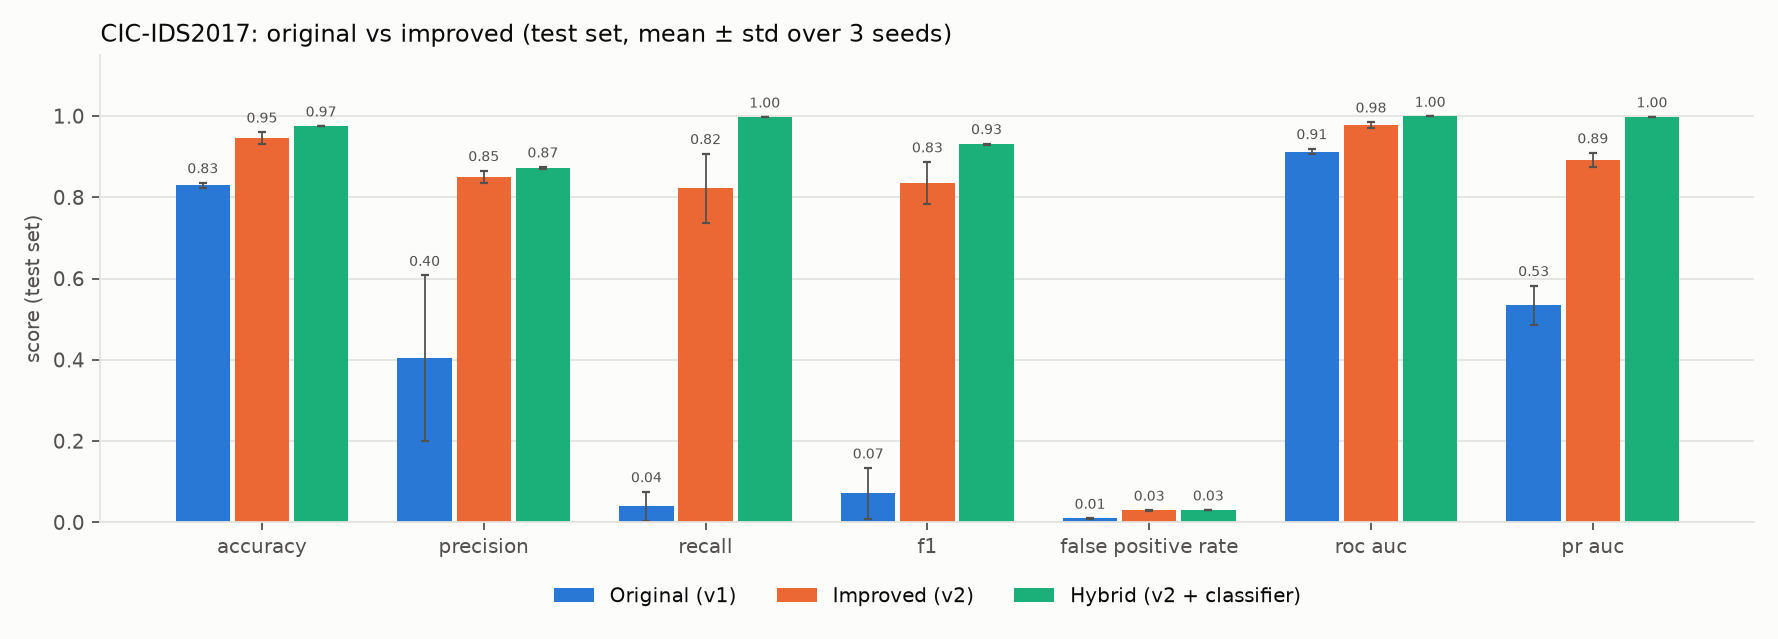
\includegraphics[width=\textwidth]{anomaly_cic_comparison.png}
\caption{Anomaly Detection on CIC-IDS2017: original vs.\ improved vs.\ hybrid (test set, mean $\pm$ standard deviation over three seeds)}
\label{fig:ad-results}
\end{figure}

\textbf{Limitations.} The rise in false positives on NSL-KDD comes from a known difference between the normal traffic in its training and test files. The training false-positive rate was 4.6\%, against 11.8\% on test, so thresholds will need recalibration on each deployment network. On CIC-IDS2017, the v2 detector still rarely detects SSH-Patator, web attacks and Bot traffic, which look statistically similar to normal flows. The F1-score of v2 on CIC-IDS2017 varied between 0.776 and 0.876 across seeds. Tuning used a single validation split instead of cross-validation. Before this protocol was fixed, an early exploratory analysis had examined CIC-IDS2017 test results; this is disclosed as a possible source of bias.

\subsection{Relationship Between the Modules}
\label{sec:module-relationship}

The three modules address different parts of the same defensive task. Network Threat Classification and Malware Classification are supervised. They are precise on the attack families and malware categories present in their training data, but they cannot recognise genuinely new behaviour. Anomaly Detection is unsupervised, so it is less precise but can flag behaviour that has never been labelled. The anomaly module's evaluation supports this division of labour: its supervised component lifted recall on known CIC-IDS2017 attacks from 82\% to 99.7\%, while on unseen NSL-KDD attacks the unsupervised detector provided almost all of the coverage. In the integrated system, the network classifier is expected to take the supervised role for flows and the anomaly detector the unsupervised role, and their outputs will be combined by the planned correlation component. This combination has not yet been implemented or tested.

Two points must be kept in mind when comparing the modules. First, the network classifier also produces an Isolation Forest anomaly score. That score is an unvalidated auxiliary signal, whereas the Anomaly Detection module is the dedicated, evaluated component for this task. Second, both flow modules use CIC-IDS2017 but with different protocols. The network module keeps duplicate flows (grouped within one partition) and uses the full dataset, while the anomaly module removes duplicates and uses a 10\% sample. Their numbers are therefore not directly comparable, and the integration phase will need a common evaluation split.

\subsection{Planned Components}

Table~\ref{tab:status} summarises the implementation status of all proposed components. Log analysis is under development. The backend API and database (FastAPI and a relational database are planned), the dashboard (React is planned), incident correlation, risk analysis and the investigation agent will be developed in later increments. The agent will follow the main steps of incident handling described in NIST guidance \cite{nist80061r3}.

\begin{table}[H]
\centering
\caption{Implementation status of the proposed components at mid-term}
\label{tab:status}
\small
\begin{tabular}{lll}
\toprule
\textbf{Component} & \textbf{Status} & \textbf{Current form} \\
\midrule
Network Threat Classification & Completed & Prototype; CLI and Python API \\
Malware Classification & Completed & Prototype; Gradio interface \\
Anomaly Detection & Completed & Prototype; CLI and Python API \\
Log Analysis & In progress & Under development \\
Network Monitoring (live capture) & Planned & -- \\
Incident Correlation & Planned & -- \\
Vulnerability Analysis & Planned & -- \\
Attack-Path Analysis & Planned & -- \\
Attack Prediction & Planned & -- \\
Risk Analysis & Planned & -- \\
Investigation Agent & Planned & -- \\
Dashboard and Feedback & Planned & -- \\
Integration backend and database & Planned & -- \\
\bottomrule
\end{tabular}
\end{table}

\subsection{Design Considerations}

\textbf{User interface and experience.} The planned dashboard will group alerts into incidents and show, for each one, the module that raised it, its severity, its confidence and the features behind it. The aim is that an analyst can understand an alert without opening several tools. The Gradio interface of the malware module is an early example of this approach.

\textbf{Technical implementation.} All modules are implemented in Python with widely used libraries, and each saves its trained models and preprocessing objects so that it can be reloaded for inference without retraining. The planned backend will expose each module through a common interface, so that adding or replacing a model does not affect the others.

\textbf{Security and data privacy.} The modules are trained only on public datasets and store no personal data. In a deployment, flow records and logs may contain sensitive information, so the planned backend will need access control, and stored results will need protection. The decision to produce response recommendations instead of executing them is also a safety measure, since an incorrect automatic block could disrupt legitimate services.

\textbf{Customisation and flexibility.} Thresholds, detector choices and model settings are kept in configuration files rather than in code. The anomaly module, for example, stores its tuned settings for each dataset in YAML files. An organisation can therefore adjust its false-alarm budget or retrain a module on its own data.

\textbf{Anticipated impact.} The completed modules show that the platform can give specific labels for known network attacks and malware, and can still flag a large share of previously unseen attacks. Once integrated, these results should reduce the time analysts spend on initial triage, provided that the models are validated on the target network first.
